\documentclass[10pt]{article}
\usepackage{ctex}
\usepackage{CJK}
\usepackage{graphicx}
\bibliographystyle{plain}
\setlength{\parindent}{2em}
\begin{document}
\title{Chinese science and technology}
\author{Qilei Zhang}
\date{may 19 2018}
\maketitle
\par
\begin{figure}[htbp]
\small
\centering
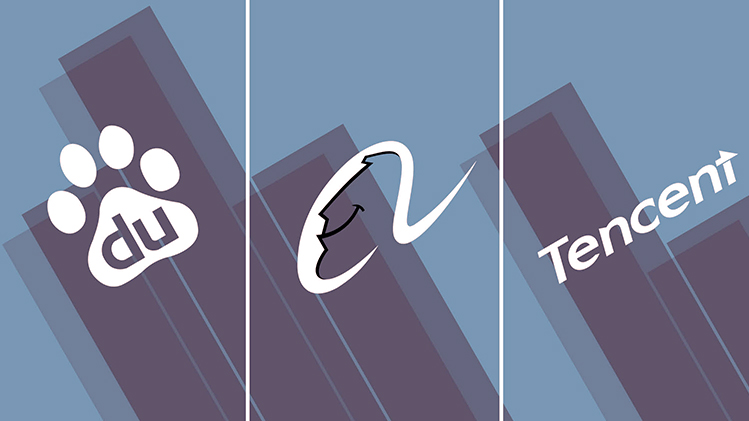
\includegraphics[width=20em]{baidu.jpg}
\caption{Figure:Chinese science and technology giants }
\label{fig:lable}
\end{figure}
\par
\section{background}
As the quest to master artificial intelligence intensifies, China��s tech trio of Baidu, Alibaba and Tencent have a distinct advantage over their Silicon Valley rivals �� data. Baidu, Alibaba and Tencent, have embraced AI with alacrity: setting up specialist labs at home and overseas and hiring top engineers. Much like their US peers such as Google, they are using machine learning to push into newer fields of autonomous driving, medical diagnosis, facial recognition for payments and AI-enabled hardware that can be operated by voice.\cite{higham1994bibtex}
\par
\section{text}
The business industry is still in its infancy in the use of AI, but this kind of application suggests how China can lead the world, especially as companies speed up the use of related technologies.\cite{h1994bibtex}
\par
Smarter AI and bigger data caches apply to medical applications too. Tencent is planning to apply this technology to the detection of early lung cancer. All industries can combine with AI and play a more efficient role.
\par
\bibliography{aaa}
\footnote{\centering Chinese science and technology}
\end{document}

